\documentclass[11pt,a4paper]{article}
\usepackage{tikz}
\usetikzlibrary{arrows.meta,positioning}
\usepackage{tabularx}
\usepackage{amsmath,amssymb,amsthm}
\usepackage{geometry}
\geometry{margin=1in}
\usepackage{hyperref}
\usepackage{graphicx}
\usepackage{setspace}
\onehalfspacing

\title{\textbf{Paper B-06: Urban Systems and Infrastructure:\\ A Constraint-Driven Flux Dynamics (CDFD) Perspective}}
\author{Steve Bico Mujjabi, MD\\
\small Independent Researcher\\
\small Founder, Vura Labs\\
\small Kampala, Uganda\\
\small ORCID: 0009-0001-0556-5516}
\date{August 2026}

\begin{document}
\maketitle

% BEGIN SHARED-METHODS POINTER
\noindent\textit{Shared Part IV notation and evidence boundaries are defined in \path{PART_IV_METHODS_AND_CLAIM_BOUNDARY.md}. This paper states only its local observables, comparison, and failure conditions.}
% END SHARED-METHODS POINTER


\begin{abstract}
This paper develops a falsifiable CDFD/AFL model of Urban Infrastructure. It maps mobility, water, energy, waste, housing, and communication demand to driving flux $\Phi$, road, pipe, grid, land, fiscal, and governance capacity to active constraint $C$, multimodal routing, maintenance, planning, pricing, and mutual aid to responsiveness $S$, and built form, segregation, deferred maintenance, and investment history to structural memory $M_s$. The target outcome is access, reliability, congestion, health, and recovery, tested against mobility traces, utility telemetry, land use, budgets, service access, and incident records. The paper treats universality as a shared model architecture rather than an assertion that unlike systems have the same material mechanism. It states the negative result that would make the mapping unnecessary and places the domain claim inside the cumulative CDFD programme and its reproducible runtime boundary.
\end{abstract}
% BEGIN CONSOLIDATION SCOPE
\section*{Consolidation Scope and Provenance}
This consolidated paper incorporates infrastructure and social urban-system scopes formerly carried by Papers B-06 and C-05. Service delivery, mobility, housing, and social recovery require separate observable tables and native baselines.
% END CONSOLIDATION SCOPE


\section{Introduction}

A city is a macroscopic metabolic engine. It inhales electricity, food, and human capital, and exhales waste, innovation, and manufactured goods. The efficiency of a city is dictated entirely by its transport networks: roads, subways, water mains, and fiber optics.

When urban planners design a city, they are effectively designing the initial topological constraints for this fluid dynamic system. Under CDFD, urban scaling laws (such as sublinear scaling of infrastructure and superlinear scaling of GDP) are naturally derived from the adaptive relationship between systemic flow and structural friction.

\section{The Urban Adaptive Surface}
We govern the urban metabolism using the Adaptive Operating Ratio:
\begin{equation}
    \Psi_s = \left( \frac{\Phi}{C} \right) \cdot S \cdot M_s
\end{equation}

For a specific city or metropolitan sector:
\begin{itemize}
    \item \textbf{Flux ($\Phi$)}: The daily volume of traffic, resource delivery, and economic transactions flowing through the sector.
    \item \textbf{Constraint ($C$)}: The physical limitations of the roads (number of lanes), zoning restrictions, and the friction of spatial distance.
    \item \textbf{Responsiveness ($S$)}: The public transit elasticity and the ability to dynamically reroute traffic or change land-use designations.
    \item \textbf{Memory ($M_s$)}: The physical built environment. Once skyscrapers and highways are poured in concrete, the city's topology is essentially locked. The high $M_s$ of a mature city prevents smooth adaptation to changing socioeconomic trends.
\end{itemize}

\subsection{Gridlock and Urban Decay}
In a young, developing city, constraints are low and responsiveness is high. The city rapidly absorbs new population flux, remaining in a healthy growth regime ($\Psi_s > 1$).

As the city matures, the concrete infrastructure locks the spatial topology ($M_s \to 1.0$). If the population (and thus the commuter flux $\Phi$) continues to grow, the fixed constraints $C$ are overwhelmed. Traffic jams become permanent; housing prices skyrocket due to zoning limits. The adaptive ratio plummets ($\Psi_s \ll 1$). The city enters an "ischemic" state of gridlock. Economic vitality chokes because the systemic memory prevents the topology from flexing.

To restore equilibrium, the city cannot rely on smooth adaptation. It must engage in massive, disruptive topological surgery: demolishing entire neighborhoods to build new transit lines or abandoning decaying sectors altogether (Detroit, Rust Belt phenomena). This is the urban equivalent of surgical amputation to remove necrotic, over-constrained tissue.



\section{Measurement Layer}

% BEGIN PART IV MAJOR CROSS-DOMAIN UPGRADE
\section{Cross-Domain Model Upgrade: Mechanism, Scale, and Tests}

\subsection{Observable Translation}

The paper-specific translation begins with an observable chain rather than a
verbal analogy. For Urban Infrastructure, the proposed drive is mobility, water, energy, waste, housing, and communication demand.
The active limitation is road, pipe, grid, land, fiscal, and governance capacity. Responsiveness is carried by
multimodal routing, maintenance, planning, pricing, and mutual aid, while retained state is represented by
built form, segregation, deferred maintenance, and investment history. The outcome to explain is access, reliability, congestion, health, and recovery.

\begin{table}[htbp]
\centering
\small
\caption{Operational CDFD/AFL map for Paper B-06.}
\begin{tabularx}{\textwidth}{|l|X|X|}
\hline
\textbf{Term} & \textbf{Paper-specific observable meaning} & \textbf{Measurement question} \\
\hline
$\Phi$ & mobility, water, energy, waste, housing, and communication demand & What rate, load, gradient, or demand enters the focal system? \\
\hline
$C$ & road, pipe, grid, land, fiscal, and governance capacity & Which measured bottleneck limits transfer, function, or recovery? \\
\hline
$S$ & multimodal routing, maintenance, planning, pricing, and mutual aid & Which process changes effective capacity or reroutes the load? \\
\hline
$M_s$ & built form, segregation, deferred maintenance, and investment history & Which retained state makes equal present loads produce different futures? \\
\hline
$Y$ & access, reliability, congestion, health, and recovery & Which outcome is predicted out of sample, with uncertainty? \\
\hline
\end{tabularx}
\end{table}

\begin{figure}[htbp]
\centering
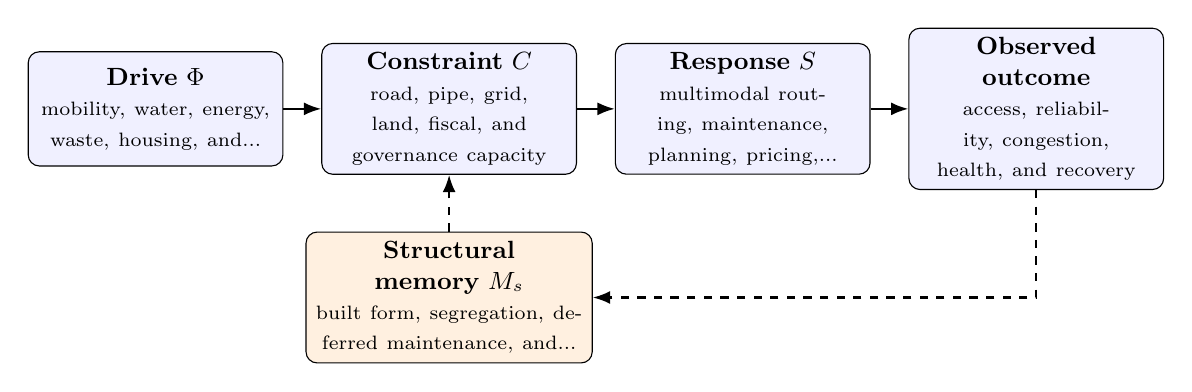
\begin{tikzpicture}[
    node distance=0.48cm,
    every node/.style={font=\small},
    box/.style={draw, rounded corners, align=center, minimum height=1.45cm, text width=3.0cm, fill=blue!6},
    memory/.style={draw, rounded corners, align=center, minimum height=1.25cm, text width=3.4cm, fill=orange!12},
    flow/.style={-{Latex[length=2.2mm]}, thick},
    feedback/.style={-{Latex[length=2.2mm]}, thick, dashed}
]
\node[box] (drive) {\textbf{Drive $\Phi$}\\\scriptsize mobility, water, energy, waste, housing, and...};
\node[box, right=of drive] (constraint) {\textbf{Constraint $C$}\\\scriptsize road, pipe, grid, land, fiscal, and governance capacity};
\node[box, right=of constraint] (response) {\textbf{Response $S$}\\\scriptsize multimodal routing, maintenance, planning, pricing,...};
\node[box, right=of response] (outcome) {\textbf{Observed outcome}\\\scriptsize access, reliability, congestion, health, and recovery};
\node[memory, below=0.72cm of constraint] (memory) {\textbf{Structural memory $M_s$}\\\scriptsize built form, segregation, deferred maintenance, and...};
\draw[flow] (drive) -- (constraint);
\draw[flow] (constraint) -- (response);
\draw[flow] (response) -- (outcome);
\draw[feedback] (outcome.south) |- (memory.east);
\draw[feedback] (memory.north) -- (constraint.south);
\end{tikzpicture}
\caption{Paper B-06 observable CDFD/AFL architecture for Urban Infrastructure. Solid arrows give the proposed forward chain; dashed arrows make history-dependent feedback explicit.}
\label{fig:b06-architecture}
\end{figure}

\subsection{Paper-Specific Causal Hypothesis}

For this paper, the hypothesized causal sequence is specific. A change in
mobility, water, energy, waste, housing, and communication demand arrives faster than multimodal routing, maintenance, planning, pricing, and mutual aid can compensate.
This raises or redistributes road, pipe, grid, land, fiscal, and governance capacity. If the load persists,
the retained state encoded by built form, segregation, deferred maintenance, and investment history changes the next response, so a later event of equal
magnitude can produce a different trajectory in access, reliability, congestion, health, and recovery. The
scientific task is to estimate that sequence against the best ordinary model of
the domain, not merely to redescribe the outcome after it occurs.

\subsection{Cross-Scale Translation Without Mechanistic Erasure}

For the engineered systems family, the cross-domain translation compares demand, designed capacity, feedback control, dependency topology, and accumulated technical state. The strongest engineering use is prospective: the mapping must identify a bottleneck, a control action, or a recovery signature before the failure occurs. \cite{BarabasiAlbert1999,WattsStrogatz1998,Shannon1948,BakTangWiesenfeld1987}
The required scale declaration for this paper is minutes to centuries; blocks to metropolitan regions. At short
scales, the key question is whether the incoming drive is transmitted,
buffered, or diverted. At intermediate scales, response changes effective
capacity and network exposure. At long scales, retained structure can alter the
state space itself. A result is genuinely cross-scale only when the aggregation
rule is stated and the same conclusion is not an artifact of averaging.

\subsection{Evidence Ladder and Discriminating Tests}

\begin{table}[htbp]
\centering
\small
\caption{Evidence ladder for Paper B-06. Each rung can fail independently.}
\begin{tabularx}{\textwidth}{|p{0.17\textwidth}|X|X|}
\hline
\textbf{Test} & \textbf{Design} & \textbf{Discriminating result} \\
\hline
Proxy audit & Measure mobility traces, utility telemetry, land use, budgets, service access, and incident records and preregister how each record maps to $\Phi$, $C$, $S$, $M_s$, and $Y$. & The mapping fails if proxies are non-identifiable, circular, or change meaning across cases. \\
\hline
Load ramp & Apply or observe a heat, flood, or demand shock across coupled urban services while estimating the dominant constraint and response time. & A threshold claim requires a reproducible nonlinear change and uncertainty bounds, not a visually chosen breakpoint. \\
\hline
Recovery and memory & Match present load across units with different histories, then compare recovery paths. & The memory claim requires history-dependent divergence after current conditions are controlled. \\
\hline
Model comparison & Compare the baseline domain model with and without the CDFD/AFL state variables using held-out data. & The paper's stated falsifier is: the framework cannot identify failures or inequities beyond ordinary urban models. \\
\hline
\end{tabularx}
\end{table}

\subsection{Research Programme and Boundary Conditions}

The immediate research programme has four steps. First, construct a documented
dataset from mobility traces, utility telemetry, land use, budgets, service access, and incident records and retain raw units before normalization.
Second, fit a baseline domain model and report its calibration and out-of-sample
error. Third, add the smallest identifiable CDFD/AFL state extension and test
whether it improves prediction of access, reliability, congestion, health, and recovery. Fourth, repeat the
analysis across the declared scale range and publish negative cases as part of
the cross-domain translation audit.

% END PART IV MAJOR CROSS-DOMAIN UPGRADE

\section{Conclusion}
Urban planning is fundamentally a discipline of thermodynamic constraint management. A city is a biological cell written in steel and glass. By modeling urban environments through the CDFD ontology, we realize that rigid infrastructure is a fatal memory trap, and sustainable cities must prioritize extreme topological responsiveness to avoid model-predicted gridlock.
\section*{Conflict of Interest} The author declares no conflict of interest.
\section*{Data Availability}
Part-specific runtime diagnostics are under each Part's \path{outputs/} directory.

Release-wide code: \path{Part_E_Synthesis/supplementary/}.

Generated summaries: \path{Part_E_Synthesis/outputs/}.

Figures: \path{Part_E_Synthesis/figures/}.


\section{Reference Layer}
\bibliographystyle{plain}
\bibliography{universal_afl_references}
\end{document}
